%%%%%%%%%%%%%%%%%%%%%%%%%%%%%%%%%%%%%%%%%
% Tufte-Style Book (Documentation Template)
% LaTeX Template
% Version 1.0 (5/1/13)
%
% This template has been downloaded from:
% http://www.LaTeXTemplates.com
%
% Original author:
% The Tufte-LaTeX Developers (tufte-latex.googlecode.com)
%
% License:
% Apache License (Version 2.0)
%
% IMPORTANT NOTE:
% In addition to running BibTeX to compile the reference list from the .bib
% file, you will need to run MakeIndex to compile the index at the end of the
% document.
%
%%%%%%%%%%%%%%%%%%%%%%%%%%%%%%%%%%%%%%%%%

%----------------------------------------------------------------------------------------
%	PACKAGES AND OTHER DOCUMENT CONFIGURATIONS
%----------------------------------------------------------------------------------------

\documentclass{tufte-book} % Use the tufte-book class which in turn uses the tufte-common class

\hypersetup{colorlinks} % Comment this line if you don't wish to have colored links
\usepackage{amsmath}
\usepackage{sudoku}
\renewcommand*\sudokuformat[1]{\sffamily #1}
\newenvironment{smallsudoku}{\setlength\sudokusize{12em}\setlength\sudokuthickline{1.5pt}\setlength\sudokuthinline{0.5pt}\begin{sudoku}}{\end{sudoku}}
\usepackage{siunitx} % align decimals in tables
\usepackage{nth}     % 1st, 2nd, ...
\usepackage{microtype} % Improves character and word spacing
\usepackage{asymptote} % for asymptote graphics
\usepackage{ccicons}
\usepackage{lipsum} % Inserts dummy text
\usepackage{booktabs} % Better horizontal rules in tables
\usepackage{graphicx} % Needed to insert images into the document

\graphicspath{{graphics/}} % Sets the default location of pictures
\setkeys{Gin}{width=\linewidth,totalheight=\textheight,keepaspectratio} % Improves figure scaling

\usepackage{fancyvrb} % Allows customization of verbatim environments
\fvset{fontsize=\normalsize} % The font size of all verbatim text can be changed here

\newcommand{\hangp}[1]{\makebox[0pt][r]{(}#1\makebox[0pt][l]{)}} % New command to create parentheses around text in tables which take up no horizontal space - this improves column spacing
\newcommand{\hangstar}{\makebox[0pt][l]{*}} % New command to create asterisks in tables which take up no horizontal space - this improves column spacing

\usepackage{xspace} % Used for printing a trailing space better than using a tilde (~) using the \xspace command

\newcommand{\monthyear}{\ifcase\month\or January\or February\or March\or April\or May\or June\or July\or August\or September\or October\or November\or December\fi\space\number\year} % A command to print the current month and year

\newcommand{\openepigraph}[2]{ % This block sets up a command for printing an epigraph with 2 arguments - the quote and the author
\begin{fullwidth}
\sffamily\large
\begin{doublespace}
\noindent\allcaps{#1}\\ % The quote
\noindent\allcaps{#2} % The author
\end{doublespace}
\end{fullwidth}
}

\newcommand{\blankpage}{\newpage\hbox{}\thispagestyle{empty}\newpage} % Command to insert a blank page

\usepackage{units} % Used for printing standard units

\newcommand{\hlred}[1]{\textcolor{Maroon}{#1}} % Print text in maroon
\newcommand{\hangleft}[1]{\makebox[0pt][r]{#1}} % Used for printing commands in the index, moves the slash left so the command name aligns with the rest of the text in the index 
\newcommand{\hairsp}{\hspace{1pt}} % Command to print a very short space
\newcommand{\ie}{\textit{i.\hairsp{}e.}\xspace} % Command to print i.e.
\newcommand{\eg}{\textit{e.\hairsp{}g.}\xspace} % Command to print e.g.
\newcommand{\na}{\quad--} % Used in tables for N/A cells
\newcommand{\measure}[3]{#1/#2$\times$\unit[#3]{pc}} % Typesets the font size, leading, and measure in the form of: 10/12x26 pc.
\newcommand{\tuftebs}{\symbol{'134}} % Command to print a backslash in tt type in OT1/T1

\providecommand{\XeLaTeX}{X\lower.5ex\hbox{\kern-0.15em\reflectbox{E}}\kern-0.1em\LaTeX}
\newcommand{\tXeLaTeX}{\XeLaTeX\index{XeLaTeX@\protect\XeLaTeX}} % Command to print the XeLaTeX logo while simultaneously adding the position to the index

\newcommand{\doccmdnoindex}[2][]{\texttt{\tuftebs#2}} % Command to print a command in texttt with a backslash of tt type without inserting the command into the index

\newcommand{\doccmddef}[2][]{\hlred{\texttt{\tuftebs#2}}\label{cmd:#2}\ifthenelse{\isempty{#1}} % Command to define a command in red and add it to the index
{ % If no package is specified, add the command to the index
\index{#2 command@\protect\hangleft{\texttt{\tuftebs}}\texttt{#2}}% Command name
}
{ % If a package is also specified as a second argument, add the command and package to the index
\index{#2 command@\protect\hangleft{\texttt{\tuftebs}}\texttt{#2} (\texttt{#1} package)}% Command name
\index{#1 package@\texttt{#1} package}\index{packages!#1@\texttt{#1}}% Package name
}}

\newcommand{\doccmd}[2][]{% Command to define a command and add it to the index
\texttt{\tuftebs#2}%
\ifthenelse{\isempty{#1}}% If no package is specified, add the command to the index
{%
\index{#2 command@\protect\hangleft{\texttt{\tuftebs}}\texttt{#2}}% Command name
}
{%
\index{#2 command@\protect\hangleft{\texttt{\tuftebs}}\texttt{#2} (\texttt{#1} package)}% Command name
\index{#1 package@\texttt{#1} package}\index{packages!#1@\texttt{#1}}% Package name
}}

% A bunch of new commands to print commands, arguments, environments, classes, etc within the text using the correct formatting
\newcommand{\docopt}[1]{\ensuremath{\langle}\textrm{\textit{#1}}\ensuremath{\rangle}}
\newcommand{\docarg}[1]{\textrm{\textit{#1}}}
\newenvironment{docspec}{\begin{quotation}\ttfamily\parskip0pt\parindent0pt\ignorespaces}{\end{quotation}}
\newcommand{\docenv}[1]{\texttt{#1}\index{#1 environment@\texttt{#1} environment}\index{environments!#1@\texttt{#1}}}
\newcommand{\docenvdef}[1]{\hlred{\texttt{#1}}\label{env:#1}\index{#1 environment@\texttt{#1} environment}\index{environments!#1@\texttt{#1}}}
\newcommand{\docpkg}[1]{\texttt{#1}\index{#1 package@\texttt{#1} package}\index{packages!#1@\texttt{#1}}}
\newcommand{\doccls}[1]{\texttt{#1}}
\newcommand{\docclsopt}[1]{\texttt{#1}\index{#1 class option@\texttt{#1} class option}\index{class options!#1@\texttt{#1}}}
\newcommand{\docclsoptdef}[1]{\hlred{\texttt{#1}}\label{clsopt:#1}\index{#1 class option@\texttt{#1} class option}\index{class options!#1@\texttt{#1}}}
\newcommand{\docmsg}[2]{\bigskip\begin{fullwidth}\noindent\ttfamily#1\end{fullwidth}\medskip\par\noindent#2}
\newcommand{\docfilehook}[2]{\texttt{#1}\index{file hooks!#2}\index{#1@\texttt{#1}}}
\newcommand{\doccounter}[1]{\texttt{#1}\index{#1 counter@\texttt{#1} counter}}

\usepackage{makeidx} % Used to generate the index
\makeindex % Generate the index which is printed at the end of the document

% This block contains a number of shortcuts used throughout the book
\newcommand{\vdqi}{\textit{VDQI}\xspace}
\newcommand{\ei}{\textit{EI}\xspace}
\newcommand{\ve}{\textit{VE}\xspace}
\newcommand{\be}{\textit{BE}\xspace}
\newcommand{\VDQI}{\textit{The Visual Display of Quantitative Information}\xspace}
\newcommand{\EI}{\textit{Envisioning Information}\xspace}
\newcommand{\VE}{\textit{Visual Explanations}\xspace}
\newcommand{\BE}{\textit{Beautiful Evidence}\xspace}
\newcommand{\TL}{Tufte-\LaTeX\xspace}

%----------------------------------------------------------------------------------------
%	BOOK META-INFORMATION
%----------------------------------------------------------------------------------------

\title{Little-$o()$ Calculus} % Title of the book

\author[W. MacEvoy]{Warren D. MacEvoy} % Author

\publisher{Lecture Notes} % Publisher

%----------------------------------------------------------------------------------------
\usepackage{ccicons}
\begin{document}

\def\asydir{graphics}
\begin{asydef}
// Global Asymptote definitions can be put here.
//import three;
//usepackage("bm");
//texpreamble("\def\V#1{\bm{#1}}");
// One can globally override the default toolbar settings here:
// settings.toolbar=true;
\end{asydef}
\frontmatter
\maketitle % Print the title page

%----------------------------------------------------------------------------------------
%	COPYRIGHT PAGE
%----------------------------------------------------------------------------------------

\newpage
\begin{fullwidth}
~\vfill
\thispagestyle{empty}
\setlength{\parindent}{0pt}
\setlength{\parskip}{\baselineskip}
Copyright \copyright\ \the\year\ \thanklessauthor

\par\smallcaps{Published by \thanklesspublisher}

\par\smallcaps{www.coloradomesa.edu}

\par \ccbyncsa\ [\url{http://creativecommons.org/licenses/by-nc-sa/4.0}]

You are free to:
\begin{itemize}
    \item Share -- copy and redistribute the material in any medium or format
    \item Adapt -- remix, transform, and build upon the material
\end{itemize}
Under the following terms:
\begin{itemize}
\item Attribution -- You must give appropriate credit, provide a link to the license, and indicate if changes were made. You may do so in any reasonable manner, but not in any way that suggests the licensor endorses you or your use.
\item NonCommercial -- You may not use the material for commercial purposes.
\item ShareAlike -- If you remix, transform, or build upon the material, you must distribute your contributions under the same license as the original. 
\end{itemize}\index{license}

\par\textit{First printing, \monthyear}
\end{fullwidth}

%----------------------------------------------------------------------------------------

\tableofcontents % Print the table of contents

%----------------------------------------------------------------------------------------

\listoffigures % Print a list of figures

%----------------------------------------------------------------------------------------

\listoftables % Print a list of tables

%----------------------------------------------------------------------------------------
%	DEDICATION PAGE
%----------------------------------------------------------------------------------------
%% \cleardoublepage
%% ~\vfill
%% \begin{doublespace}
%% \noindent\fontsize{18}{22}\selectfont\itshape
%% \nohyphenation
%% To Rose.
%% \end{doublespace}
%% \vfill
%% \vfill


%----------------------------------------------------------------------------------------
%	INTRODUCTION
%----------------------------------------------------------------------------------------
\cleardoublepage

\chapter*{Preamble}
\marginnote{Stitz-Zeager [\url{www.stitz-zeager.com}] and Boundless [\url{www.boundless.com}] are good backgrounds references.}

The point of these notes is to introduce the main concepts of calculus using what is known as little-$o()$ notation, in the hope to provide a perspective that is simple, expressive, intuitive and correct.

\section*{Algebra is essential}
\begin{marginfigure}
\begin{center}
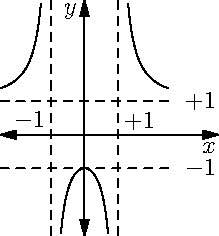
\includegraphics[width=0.75\linewidth]{graphics/algebra1.pdf}
\end{center}
\caption{$y=f(x)=\frac{x^2+1}{x^2-1}$}
\label{fig:algebra1}
\end{marginfigure}
\begin{marginfigure}
\begin{center}
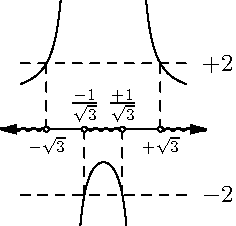
\includegraphics[width=0.75\linewidth]{graphics/algebra2.pdf}
\end{center}
\caption{Where $|f(x)|$ is less than $2$.}
\label{fig:algebra2}
\end{marginfigure}
\begin{marginfigure}
\begin{center}
\includegraphics[width=0.75\linewidth]{graphics/explog.pdf}
\end{center}
\caption{How $y=e^x$ and $x=\ln y$ are related, where $e \approx 2.72$ is Euler's constant.}
\label{fig:explog}
\end{marginfigure}

I assume you are comfortable with algebra, including working with rational algebraic expressions, exponents and logarithms, function notation, absolute values, and inequalities.

For example, seeing 

\begin{equation*}
f(x)=\frac{x^2+1}{x^2-1}
\end{equation*}

And being asked to show
\begin{equation*}
    f(x+h)=\frac{x^2+1}{x^2-1}+ \frac{2h\cdot(2x+h)}{(x-1)(x+1)(x+h+1)(x+h-1)}
\end{equation*}
and
\begin{align*}
  |f(x)|<2 & \text{ if and only if } \\
           &  x \in (-\infty,-\sqrt{3})\cup(-\frac{1}{\sqrt{3}},+\frac{1}{\sqrt{3}})\cup(+\sqrt{3},+\infty)
\end{align*}
should seem (at worst) tedious, but not mysterious.  Neither should the following\footnote{Recall $b^x=e^{x \ln b}$ and $\log_b x=\ln x/\ln b$}:
\begin{equation*}
    2^{\log_3(x)}=x^{\log_2(3)} \,.
\end{equation*}

If these are mysterious to you, then you need to learn college algebra.
\newpage\section*{Trigonometry is helpful}
\begin{marginfigure}
\begin{center}
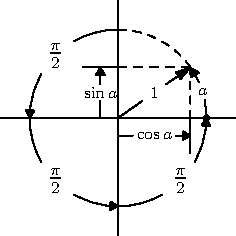
\includegraphics[width=0.75\linewidth]{graphics/unitcircle.pdf}
\end{center}
\caption{Defining $\cos a$ and $\sin a$ for radian angle $a$ on the unit circle. Notice there are $2\pi \approx 6.28$ radians in a circle.}
\label{fig:unitcircle}
\end{marginfigure}
It will be useful if you have some basic trigonometry, including measuring angles in radians, which is the only unit of angle we care about here.  For example,
\begin{gather*}
    (\cos a)^2 +(\sin a)^2 = 1\,,\\
    \cos a=
        \frac{1}{2}\text{ if and only if $a=\pm\frac{\pi}{3}+2\pi n$, for some integer $n$}\,,
\intertext{and}
    \sin(a + b)=\sin(a) \cos(b) + \cos(a) \sin(b)\,, \\
    \cos(a + b)=\cos(a) \cos(b) - \sin(a) \sin(b)\,, \\
\end{gather*}
should at least be familiar to the point of looking something up to remember the details.

\begin{marginfigure}
\begin{smallsudoku} % -- simple
| | |6|1| |5| | | |.
|9| | | |4| |7| | |.
|8| | |7| | | |2| |.
|4| | | | | | | | |.
| | |1| | | |4| | |.
| | | | |6| | | | |.
| |5| |8| |2|1| | |.
| |6| | | |9| | |7|.
| |4| | | |6|9| |5|.
\end{smallsudoku}
\caption{A simple sudoku puzzle.  Each row, column and $3 \times 3$ subgrid must contains all of the digits from 1 to 9.}
\label{fig:sudoku-simple}
\end{marginfigure}
\section*{Reading Tips}
\begin{marginfigure}
\begin{center}
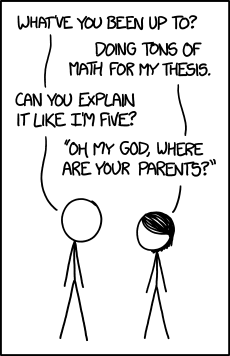
\includegraphics{graphics/like_im_five.png}
\end{center}
\caption{\url{http://xkcd.com/1364}}
\label{fig:xkcd1364}
\end{marginfigure}
\begin{itemize}
\item Focus. The best environment for learning something mathematical is in a small group willing to help you work out a sudoku puzzle.  If you can work out a sudoku puzzle in the place and with the people you study with, it is a good sign you can learn math as well.  Learning, any learning, is for mono-taskers: you might multitask (usually poorly) on things you already understand.  This, however, is something you are trying to understand.
\item Drive, don't walk. Learning to use a computer algebra system (like Wolfram Alpha, wxMaxima or Maple), or at least a spreadsheet (like Google Docs, Libre Office or Microsoft Excel) can spare you from a lot of tedium compared to a crummy calculator.
\item Understand first. Proofs are less important than understanding.  If you are mostly interested in applications, don't worry as much about understanding every proof.  Concentrate instead on why the ideas make sense and how you might use these ideas.  If you are interested in mathematics itself, understanding the proofs is important, but useless without an intuition of why they make sense and how to use them.
\end{itemize}

\chapter{Basics}

Little-$o()$ notation is used to denote that some expression is small relative to some other value.

For example, if we say, as  $h \rightarrow 0$ (as $h$ approaches zero),  
\begin{equation} 
(1 + h)^3 = 1 + 3 h + o(h)\,.
\end{equation}

\begin{marginfigure}
\includegraphics[width=0.75\linewidth]{graphics/basics1.pdf}
\caption{$(1 + h )^3$ vs.  $1 + 3 h$ for small values of  $h$.}
\label{fig:basics1}
\end{marginfigure}
We mean that the magnitude of the difference between the left-hand side  $L = (1 + h )^3$ and the  right-hand side $R = 1 + 3 h$  is so small that, even when divided by $h$,  it is still small.

We can check this ratio empirically: 
\begin{table}
\caption{$(1 + h )^3$ vs. $1 + 3 h$}
\label{tab:basic1}
\begin{tabular}{|S[table-format=2.3]|S[table-format=2.9]|S[table-format=2.3]|S[table-format=2.11]|S[table-format=2.6]|}
\multicolumn{1}{l}{$h$} & 
\multicolumn{1}{l}{$L = (1 + h )^3$} & 
\multicolumn{1}{l}{$R = 1 + 3 h$} & 
\multicolumn{1}{l}{$E = L - R$} &
\multicolumn{1}{l}{$r = \left| \frac{E}{h} \right| $} \\
\hline
0.1  & 1.331 & 1.3 & 0.031 & 0.31 \\
\hline
-0.01 & 0.970299 & 0.97 & 0.000299 & 0.0299 \\
\hline
0.001 & 1.003003001 & 1.003 & 0.00000030001 & 0.003001 \\
\hline
\end{tabular}
\end{table}

Notice how the ratio  $r=|E/h|$ shrinks as the magnitude of  
$h$ shrinks.  When we say an expression  $E$  is 
$o(h)$ as  $h \rightarrow 0$,  we mean the magnitude of $|E/h|$  gets small as the magnitude of $h$ gets small.  
 
The  $o()$  notation allows for more general expressions for the relative comparison of smallness,  such as  $o(h^2)$ or  $o(h \ln(h))$. In each case, we are saying that the expression in question is small in magnitude when divided by the expression in the $o()$  as the parameter ($h$ in this case) gets small in magnitude.

Here are some other examples to help get the idea.  You should check these with a calculator or spreadsheet.  We give a formal definition of the notation at the end of this section. 
 
As  $k \rightarrow \infty$,  $2k^3 + 5 k^2 - 7 k + 3 = 2k^3 + o (k^3 )$.     
 
This means, as the magnitude of  $k$ gets larger and larger, the cubic polynomial on the left is approximately the leading order term (term with the highest power of  $k$) plus an error small relative to the size of that term.   

\begin{table}
\caption{$2k^3 + 5 k^2 - 7 k + 3$ vs. $2k^3$.}
\label{tab:basic2}
\begin{tabular}{|S[table-format=4]|S[table-format=10]|S[table-format=10]|S[table-format=7]|S[table-format=10]|S[table-format=1.5]|}
\multicolumn{6}{c}{\vspace{1em}} \\
\multicolumn{1}{l}{$k$} & 
\multicolumn{1}{l}{$\begin{array}{c}L=2k^3+ 5 k^2 \\ - 7 k + 3\end{array}$} & 
\multicolumn{1}{l}{$R=2k^3$} & 
\multicolumn{1}{l}{$E=L-R$} &
\multicolumn{1}{l}{$\varepsilon(k)=k^3$} &
\multicolumn{1}{l}{$r=\left|\frac{E}{\varepsilon(k)}\right| $} \\
\hline
10  & 2433 & 2000 & 433 & 1000 & 0.43300 \\
-100 & -1949297 &  -2000000 & 50703 & -1000000 & 0.05070 \\
1000 & 2004993003 & 2000000000 & 4993003 & 1000000000 & 0.00499 \\
\hline
\end{tabular}
\end{table}

Notice how the error $E$ grows, but it is still small when compared to $\varepsilon(k) = k^3$.  

\section{$e$}
As $h \rightarrow 0$, $(1 + h)^{1/h}=e+o(h^0)$.

This means, as the magnitude of  $h$ gets smaller and smaller, the expression on the left is  
approximately Euler's constant $e = \num{2.718281828459045}\ldots$, plus an error small relative to $h^0=1$.

Just as  $\pi$ plays a fundamental role in trigonometry, $e$ is fundamental for exponents and  
logarithms. 
\begin{marginfigure}
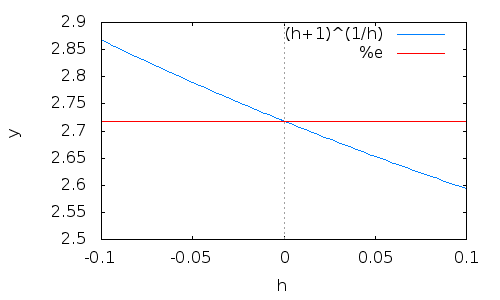
\includegraphics[width=0.75\linewidth]{graphics/e.pdf}
\caption{$(1 + h )^{1/h}=e+o(h^0)$.}
\label{fig:basics1}
\end{marginfigure}
 
Here is a tabular comparison for some small values of  h :  
 
\begin{table}
\caption{$2k^3 + 5 k^2 - 7 k + 3$ vs. $2k^3$.}
\label{tab:basic2}
\begin{tabular}{|S[table-format=2.6]|S[table-format=1.8]|S[table-format=1.8]|S[table-format=7]|S[table-format=10]|S[table-format=1.5]|}
\multicolumn{6}{c}{\vspace{1em}} \\
\multicolumn{1}{l}{$h$} & 
\multicolumn{1}{l}{$L=(1+h)^{1/h}$}
\multicolumn{1}{l}{$R=e2k^3$} & 
\multicolumn{1}{l}{$E=L-R$} &
\multicolumn{1}{l}{$\varepsilon(h)=h^0$} &
\multicolumn{1}{l}{$r=\left|\frac{E}{\varepsilon(h)}\right| $} \\
\hline
ε (h) = h 0   E |  
r = || ε(k)
|
2.7182818...  -0.0135  1  0.0135 
2.718417755  2.7182818...  0.000136  1  0.000136 
2.718280469  2.7182818...  -0.00000136  1  0.00000136 
h   L = (1 + h ) 1/h   R = e  
0.01  2.704813829  -0.0001  0.000001 
E = L − R   
 
Writing 1 as  h 0 in the  o () may seem surprising, but it is a way of noting what parameter is getting  
small.   
 
As  h → 0   ,  s in(x + h ) = s in(x) + c os(x)h + o (h) .    
 
We will show this is true later, but, geometrically, it means that evaluating  s in(x) near  x is  
approximately a line going through the point  ( x, s in(x)) with slope  c os(x).  
 
Here is a plot of these approximations for  s in(x) at  x = 1 , 2 , and  3 :   
 
This last example is really important.  The idea that, near a given point  x ,  many functions  
are well approximated by a line is a foundational idea of differential calculus.  We call the 
slope of that approximating  line  f ′ (x) , so that  f (x + h ) = f (x) + f ′ (x)h + o (h) .  For this example, we  
are saying that, if  f (x) = s in(x) , then  f ′ (x) = c os(x) .  
 
 
Figure 1.  The most important figure in calculus.  For many functions, the value near a given point  x is well approximated by a line called the tangent line of  f (x)  at  x with slope  f ′ (x).     As an  
equation: as  h → 0 ,   f (x + h ) = f (x) + f ′ (x)h + o (h).     Such functions are called differentiable at  x .  
 
Always writing “as  h → 0 "  is tedious.  It will be clear from the  o ()  notation which parameter we  
consider large or small. 
 
Formalities
E | is as small as we choose,  
An expression  E    is  o (ε(h))  as  h → 0 , means the ratio  r = || ε(h)
|
provided we force the magnitude of  h to be small enough (but not zero).  Specifically, for  
E | < r .  
any bound   r b > 0 ,  there exists an 
 
h b > 0 ,  so that, if  0 < | h | < h b ,  then  || ε(h)
| b
 
 
 
 
Redraw this in your notes so you remember the definition of little-o. 
 
 
E | = 0 .  
If you are familiar with limit notation, this can be written as  lim || ε(h)
|
h→0
 In terms of large parameters,  E = o (ε(k))    as  k → ∞   is the same as  E = o (ε(1/h))  as
   
h → 0 by means of the substitution  h = 1 /k.  
 
E | = 0 .  
If you are familiar with limit notation, this can be written as  lim || ε(k)
|
k→∞
 
Note that we divide  E  by 
  ε (h)  to get  r  in the above definition for some range of nonzero
 
 
values of  h .    So, for for any expression to be  o (ε(h)),   ε (h)  must be defined and nonzero  
for some range of nonzero values of  h .    We therefore restrict  ε (h)  to such admissible  
functions:   
 
For  ε (h)  to be admissible in  o (ε(h))  notation, there must exist some  h ε > 0  so  
that  ε (h)  is defined (finite) and nonzero for  0 < | h | < h ε .     
 
 
All we ask of  ε (h)  to be admissible, is that there is a range near zero (but we don’t  
care about at zero), where it is defined (finite) and nonzero.  This way we can 
divide  E    by  ε (h)  in this range to compute the ratio  r = | E/ε(h)|.  
 
 We only use admissible   ε (h)  in these notes.  In particular,  ε (h) = | h | p  is admissible for  
any value of  p ,  and   ε (h) = h p  is admissible for any integer value of  p .  
Summary
 
●
Little-o() notation is a way of describing an expression as small in comparison to 
some other value: saying  E  is 
  o (ε(h))  as  h → 0  means the ratio  r = | E/ε(h) |  can
 
 be made as small as desired provided the magnitude of  h is small enough (but  
not zero). 
 
●
Specifically,  E    is  o (ε(h))  as  h → 0  means:  
 
For any  r b > 0 ,  there exists 
 
h b > 0 ,  so that:   
E | < r .  
|
 If  0 < | h | < h b ,  then  | ε(h)
| b
 
● E  is 
  o (ε(k))    as  k → ∞   means  E is 
  o (ε(1/h))  as  h = 1 /k → 0 .  
● For differentiable functions, the value  f (x + h )  near a given point  x is well  
approximated by a line called the tangent line of  f (x)  at  x with slope  f ′ (x).    
● As  h → 0 ,   (1 + h ) (1/h) = e + o (h 0 ),  where  e ≈ 2 .718  is Euler’s constant.
 
 
● Because an expression  E  is divided by 
 
ε (h) in the definition of  o (ε(h)),   ε (h)  is  
admissible in  o (ε(h))  only if it is defined and nonzero for small enough nonzero  
h :  there must exist  h ε > 0  so that  ε (h)  is defined (finite) and nonzero for  
0 < | h | < h ε .     
●  We only use admissible   ε (h)  in these notes.  In particular,  ε (h) = | h | p  is  
admissible for any value of  p ,  and   ε (h) = h p  is admissible for any integer value of  
p .  


\backmatter

\bibliography{bibliography} % Use the bibliography.bib file for the bibliography
\bibliographystyle{plainnat} % Use the plainnat style of referencing
\printindex % Print the index at the very end of the document

\end{document}
